\documentclass[11pt, a4paper]{article}
\usepackage{graphicx, fullpage, hyperref, listings}
\usepackage{appendix, pdfpages, color}

\usepackage{tocloft}            % This squashes the Table of Contents a bit
\setlength\cftbeforesecskip{3pt}

\definecolor{MyLightYellow}{cmyk}{0,0.,0.2,0}

\setlength{\parskip}{4pt}        % sets spacing between paragraphs
\interfootnotelinepenalty=500    % this prevents footnotes breaking across pages

\title{
\includegraphics[width=0.4\textwidth]{UnivCrest}
        \\Experiment 22 - Monte Carlo Simulation}          % <<<<<<<<< change the title as appropriate
\author{%\textcolor{red}{Student ID 200123456 (Group 999)}                % <<<<<<<<< your ID and group number
        \\  \textcolor{red}{ELEC273}\footnote{\textcolor{red}{IMPORTANT: In a standard technical report, you would need to include here your personal details as the author of the document. However, remember that marking of coursework is anonymous and therefore you should remove this part before submitting your report for Year 2 labs! Do not include your name, student ID, email address or any other personal information.}}}                                    % <<<<<<<<< module code
\date{\tiny{\today}}

\begin{document}
\begin{titlepage}
\maketitle
\addtocontents{toc}{\protect\thispagestyle{empty}} % because we don't want a page number on the title page
                                                   % Thanks to Huang Shanyue for suggesting this

\begin{abstract}
This document describes what is expected from an engineering laboratory report. While this is not a definitive guide to report-writing, it is intended as a guide to assist in documenting and presenting your experimental work. Appended to this guide are some real examples of common mistakes that should be avoided. It is expected that lab reports are prepared using the \LaTeX~ typesetting system, adopting pne of the standard report templates provided on VITAL.
\end{abstract}

\fbox{
\begin{minipage}{0.9\linewidth} \footnotesize
\begin{center} \textbf{Declaration} \end{center}
I confirm that I have read and understood the University's definitions of plagiarism and collusion from the Code of Practice on Assessment. I confirm that I have neither committed plagiarism in the completion of this work nor have I colluded with ant other party in the preparation and production of this work. The work presented here is my own and in my own words except where I have clearly indicated and acknowledged that I have quoted or used figures from published or unpublished sources (including the web). I understand the consequences of engaging in plagiarism and collusion as described in the Code of Practice on Assessment (Appendix L).
\end{minipage}
}

\thispagestyle{empty}
\newpage
\tableofcontents
\end{titlepage}


%-------------------------------------------------------------------------------------------------------
\section{Introduction}
%-------------------------------------------------------------------------------------------------------


Include a statement of the problem to be investigated, and why is addressing this problem worthwhile or important. This section should also introduce the history and theoretical background of the problem, a brief statement of the general procedure adopted and hint at expected results. This section is sometimes broken down into subsections: Objectives and Theoretical Background.

%-------------------------------------------------------------------------------------------------------
\section{Materials and Methods}
%-------------------------------------------------------------------------------------------------------



To easily simulate penalty kicks events, a simple goal model was established according to the instruction on the lab script\cite{ref:lab}. In this experiment, Matlab was utilized to modeling the situation with pseudo random number generated with Monte Carlo algorithm.


\begin{figure}[htbp]     \begin{centering}
    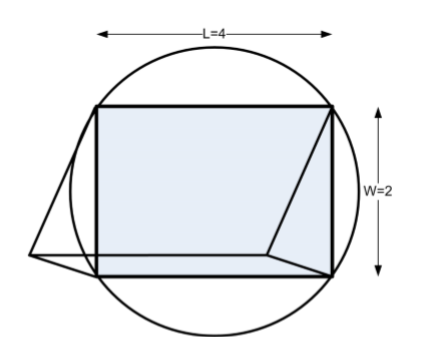
\includegraphics[width=0.5\textwidth]{goal.png}
    \caption{Goal Model (taken from~\cite{ref:lab})}
    \label{Fig:goal}
    \end{centering}
\end{figure}


It is assumed that the ball can be kicked randomly and will only fall in the circle area as it shown in Figure \ref{Fig:goal}. The distribution of balls is expected to follow certain distribution model, such as uniform distribution and normal distribution. In order to explore the distinctions between among different distribution models under diverse conditions, this experiment was designed into two parts. The first part was for the situation with no goalkeepers while the second part focused on the condition that the goalkeeper acted.

\subsection{Part 1: No Goalkeeper Tests}

In this part, the situation with no goalkeeper was modeled. Firstly, the theoretical result of the hit rate was calculated under the assumption that the distribution of balls follows uniform distribution. Secondly, Matlab was utilized to simulate this process with a uniform random number generator. Thirdly, the influence of simulating shots number N and experiment repeat times R was studied with perspectives of line charts generated with Matlab. Furthermore, the hypothesis was changed to that the distribution of balls abides by Gaussian distribution and the experiment steps above were repeated for this new assumption.

\subsection{Part 2: With Goalkeeper Tests}

\begin{figure}[htbp]     \begin{centering}
    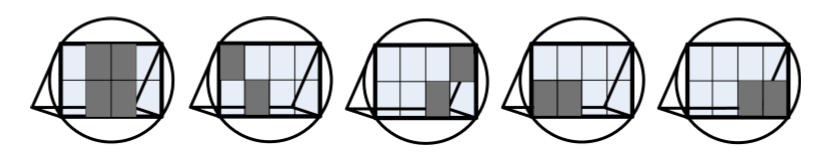
\includegraphics[width=0.5\textwidth]{goalkeeper-action.png}
    \caption{Goalkeeper Action to Penalty Shoot-outs (taken from~\cite{ref:lab})}
    \label{Fig:goalkeeper-action}
    \end{centering}
\end{figure}

Under the condition that there are goalkeeper, this football goal model can be further improved. To easily analyse the situations, the action of the goalkeeper was classified into five types ideally, as shown in Figure \ref{Fig:goalkeeper-action}. Firstly, it was considered that the possibility of these five cases was equal following uniform random distribution. Matlab was used to simulate the shooting process and then the hit rate can be figured out. Secondly, similarly with the produce in Part 1, the hypothesis was changed from uniform random distribution to Gaussian random distribution and the simulation was implemented again. Thirdly, the actions of goalkeeper was updated from equally distributed to that 90\% of the time the goalkeeper may choose position 4 and position 5. Under this circumstance, the probability of scoring was required to be simulated with kicking 100 and 1000 balls.



% You may want to use the {enumerate} environment for a numbered list.
%
%\begin{enumerate}
%    \item First numbered item
%        \subitem You can even have nested layers
%    \item Second numbered item
%    \item Third numbered item
%\end{enumerate}


%-------------------------------------------------------------------------------------------------------
\section{Results}
%-------------------------------------------------------------------------------------------------------

\subsection{Part 1: No Goalkeeper Tests}

This section presents and comments the result from the simulation with no goalkeeper.

\subsubsection{Task 1: Calculation}

In this subsection, the theoretical value of scoring probability will be calculated under the condition that balls distributed in the circle with a radius of $\sqrt{5}$ (as shown in Figure \ref{Fig:goal}) uniformly. In this case, the hit rate can be obtained through the fraction of the goal area and the circle area presented in Equation \ref{eq:posibility_by_area}.

\begin{equation}
P_{scoring} = \frac{S_{rect}}{S_{circle}}.
\label{eq:posibility_by_area}
\end{equation}

As the area of the rectangle goal is $8$ and the area of the circle zone is $5\pi$, the possibility then can be computed, which is 51.0\%.


\subsubsection{Task 2: Matlab Simulation}





This is where you describe the important qualitative and quantitative observations from the experiment. Data should be tabulated and/or graphed. Graphs must always be captioned (as with figures, above), and axes clearly annotated with units. Always follow your graphs with a brief description, demonstrating your understanding of what has been plotted (eg. ``The graph in Fig. 4 illustrates the frequency response of this circuit, with a clear resonance peak at 15~kHz.'') as tables and graphs are rarely self-explanatory. If the results differ from what was expected, explain both \textbf{how} (i.e. in what way) and \textbf{why} (i.e. possible reasons behind this behaviour) when referring to these results.

% This is how you could include a figure
%
%\begin{figure}[htbp]     \begin{centering}
%    \includegraphics[width=0.5\textwidth]{OpAmp.jpg}
%    \caption{Circuit diagram of non-inverting amplifier circuit used in Part 1 (taken from~\cite{ref:Radio})}
%    \end{centering}
%    \label{Fig:OpAmp}
%\end{figure}

% Here are some example tables

The summary of the experimental results is presented in Table~\ref{tab:summary}

\begin{table}[htbp]
\caption{Note that table captions are placed above the tables, not below as for figures}
\label{tab:summary}
\begin{center}
\begin{tabular}{ccc}
\hline
 $P$ (W)      & $V$ (V)       & $I$ (A)   \\
\hline
$0.0\pm0.01$ & $0.0\pm0.01$ & $0.0\pm0.01$  \\
 0.1         & 0.2          &  0.3         \\
 0.1         & 0.2          &  0.3         \\
 0.1         & 0.2          &  0.3         \\

\hline
\end{tabular}
\end{center}
\end{table}


\begin{table}[htbp]
\caption{Resistance and Temperature of the Filament}
\label{tab:data}
\begin{center}
\begin{tabular}{|c||c|c|c|}
\hline
$R$ ($\Omega$) & $T$ (K) & $1/T$ (K$^{-1}$) & $\ln P$ \\
\hline\hline
151.00$\pm$3.92 & 828.35$\pm$23.46& $1.2072\times10^{-3}$& -13.29 \\ \hline
157.12$\pm$3.71 & 856.88$\pm$22.25& $1.1671\times10^{-3}$& -12.64 \\ \hline
162.53$\pm$3.49 & 881.99$\pm$21.02& $1.1338\times10^{-3}$& -12.33 \\ \hline
166.67$\pm$3.33 & 901.14$\pm$20.13& $1.1097\times10^{-3}$& -11.90 \\ \hline
\hline
\end{tabular}
\end{center}
\end{table}

%------------------------------------------------------------------------------------------------------- 
\section{Discussion}
%-------------------------------------------------------------------------------------------------------

The Discussion section allows you to fully discuss and interpret the results and the results of the any analysis carried out. It is also important here to relate your findings to the experimental objectives, i.e. do your results support the theoretical background, and have the objectives of the experiment been met? Are the results reliable and/or significant?

Mathematical expressions can be included in \LaTeX documents easily by surrounding them in \verb|$| signs, such as $f$, $\delta x$, $\Omega_2$, $y=mx+b$ or $\mu = \frac{1}{N}\sum_{i=1}^N x_i$. Numbered equations can be created just as easily using the \verb|equation| environment:

\begin{equation}
\mu = \frac{1}{N}\sum_{i=1}^N x_i.
\label{eq:mean}
\end{equation}

When making reference to the above equation, you simply need to mention the label, as in ``\verb|...as shown in Equation~\ref{eq:mean}.|'', and the Equation number will be inserted automatically. If you need to show several lines of mathematical expressions, you can use the \verb|eqnarray| environment as below:

\begin{eqnarray}
  P & = & I V             \\
    & = & I^2 R           \\
    & = & \frac{V^2}{R}
\label{eq:power}
\end{eqnarray}
Further guidance on writing and manipulating mathematical expressions, symbols and equations can be found online in references such as~\cite{ref:Maths}.

%-------------------------------------------------------------------------------------------------------
\section{Conclusions}
%-------------------------------------------------------------------------------------------------------

This final section contains a brief statement to summarise the outcome of the experiment, and a statement outlining to what extent the objectives of the experiment have been met, and what has been learnt as a result of this. In some ways the Conclusions section is a reflection of the Abstract, reiterating what the experiment was aiming to achieve, and summarising the outcomes. It can also be thought of as a summary of the Discussion section.

%

%-------------------------------------------------------------------------------------------------------

\bibliographystyle{IEEEtran}
\bibliography{MyRefs}         % The file MyRefs.bib contains the actual bibliography material
                                  % References section created automatically
\addcontentsline{toc}{section}{References}



% --------------------------- This is how to declare the Appendices section ----------------------------
\newpage
\appendix
\appendixpage
\addappheadtotoc


%-------------------------------------------------------------------------------------------------------
\section{Matlab Source Code}
%-------------------------------------------------------------------------------------------------------

\subsection{Overall Structure}

This is the source code files structure instruction, which displays the list of main code files and function files.

\lstset{language=MATLAB, frame=single, basicstyle=\footnotesize, backgroundcolor=\color{MyLightYellow}, caption={Source Code Files Structure},label=tree}
\lstinputlisting[language=MATLAB]{../src/tree.js}


\subsection{Main Codes}

\subsubsection{Task 2\&3}

%-------------------------- Source code / program listings can be inserted using like this -----------
\lstset{language=MATLAB, frame=single, basicstyle=\footnotesize, backgroundcolor=\color{MyLightYellow}, caption={Matlab Source Code for Task 2},label=sct2}
\lstinputlisting[language=MATLAB]{../src/t2.m}
%-------------------------------------------------------------------------------------------------------


\subsubsection{Task 4}

%-------------------------- Source code / program listings can be inserted using like this -----------
\lstset{language=MATLAB, frame=single, basicstyle=\footnotesize, backgroundcolor=\color{MyLightYellow}, caption={Matlab Source Code for Task 4},label=sct4}
\lstinputlisting[language=MATLAB]{../src/t4.m}
%-------------------------------------------------------------------------------------------------------


\subsubsection{Task 5}

%-------------------------- Source code / program listings can be inserted using like this -----------
\lstset{language=MATLAB, frame=single, basicstyle=\footnotesize, backgroundcolor=\color{MyLightYellow}, caption={Matlab Source Code for Task 5},label=sct5}
\lstinputlisting[language=MATLAB]{../src/t5.m}
%-------------------------------------------------------------------------------------------------------


\subsubsection{Task 7}

%-------------------------- Source code / program listings can be inserted using like this -----------
\lstset{language=MATLAB, frame=single, basicstyle=\footnotesize, backgroundcolor=\color{MyLightYellow}, caption={Matlab Source Code for Task 7\_2},label=sct7_2}
\lstinputlisting[language=MATLAB]{../src/t7_2.m}
%-------------------------------------------------------------------------------------------------------

%-------------------------- Source code / program listings can be inserted using like this -----------
\lstset{language=MATLAB, frame=single, basicstyle=\footnotesize, backgroundcolor=\color{MyLightYellow}, caption={Matlab Source Code for Task 7\_4},label=sct7_4}
\lstinputlisting[language=MATLAB]{../src/t7_4.m}
%-------------------------------------------------------------------------------------------------------

%-------------------------- Source code / program listings can be inserted using like this -----------
\lstset{language=MATLAB, frame=single, basicstyle=\footnotesize, backgroundcolor=\color{MyLightYellow}, caption={Matlab Source Code for Task 7\_5},label=sct7_5}
\lstinputlisting[language=MATLAB]{../src/t7_5.m}
%-------------------------------------------------------------------------------------------------------

\subsubsection{Task 8}

%-------------------------- Source code / program listings can be inserted using like this -----------
\lstset{language=MATLAB, frame=single, basicstyle=\footnotesize, backgroundcolor=\color{MyLightYellow}, caption={Matlab Source Code for Task 8},label=sct8}
\lstinputlisting[language=MATLAB]{../src/t8.m}
%-------------------------------------------------------------------------------------------------------

\subsubsection{Task 9}

%-------------------------- Source code / program listings can be inserted using like this -----------
\lstset{language=MATLAB, frame=single, basicstyle=\footnotesize, backgroundcolor=\color{MyLightYellow}, caption={Matlab Source Code for Task 9},label=sct9}
\lstinputlisting[language=MATLAB]{../src/t9.m}
%-------------------------------------------------------------------------------------------------------

\subsubsection{Task 10}

%-------------------------- Source code / program listings can be inserted using like this -----------
\lstset{language=MATLAB, frame=single, basicstyle=\footnotesize, backgroundcolor=\color{MyLightYellow}, caption={Matlab Source Code for Task 10\_8},label=sct10_8}
\lstinputlisting[language=MATLAB]{../src/t10_8.m}
%-------------------------------------------------------------------------------------------------------


%-------------------------- Source code / program listings can be inserted using like this -----------
\lstset{language=MATLAB, frame=single, basicstyle=\footnotesize, backgroundcolor=\color{MyLightYellow}, caption={Matlab Source Code for Task 10\_9},label=sct10_9}
\lstinputlisting[language=MATLAB]{../src/t10_9.m}
%-------------------------------------------------------------------------------------------------------

\subsection{Function Codes}

\subsubsection{Draw}

%-------------------------- Source code / program listings can be inserted using like this -----------
\lstset{language=MATLAB, frame=single, basicstyle=\footnotesize, backgroundcolor=\color{MyLightYellow}, caption={Matlab Source Code for Function drawBackGround},label=scf:drawBackGround}
\lstinputlisting[language=MATLAB]{../src/func/drawBackGround.m}
%-------------------------------------------------------------------------------------------------------

\subsubsection{Math}

%-------------------------- Source code / program listings can be inserted using like this -----------
\lstset{language=MATLAB, frame=single, basicstyle=\footnotesize, backgroundcolor=\color{MyLightYellow}, caption={Matlab Source Code for Function getDisProb},label=scf:getDisProb}
\lstinputlisting[language=MATLAB]{../src/func/getDisProb.m}
%-------------------------------------------------------------------------------------------------------

\subsubsection{Tools}

%-------------------------- Source code / program listings can be inserted using like this -----------
\lstset{language=MATLAB, frame=single, basicstyle=\footnotesize, backgroundcolor=\color{MyLightYellow}, caption={Matlab Source Code for Function getDisProb},label=scf:getDisProb}
\lstinputlisting[language=MATLAB]{../src/func/getDivByPos.m}
%-------------------------------------------------------------------------------------------------------

%-------------------------- Source code / program listings can be inserted using like this -----------
\lstset{language=MATLAB, frame=single, basicstyle=\footnotesize, backgroundcolor=\color{MyLightYellow}, caption={Matlab Source Code for Function isGoalKept},label=scf:isGoalKept}
\lstinputlisting[language=MATLAB]{../src/func/isGoalKept.m}
%-------------------------------------------------------------------------------------------------------

%-------------------------- Source code / program listings can be inserted using like this -----------
\lstset{language=MATLAB, frame=single, basicstyle=\footnotesize, backgroundcolor=\color{MyLightYellow}, caption={Matlab Source Code for Function isInRect},label=scf:isInRect}
\lstinputlisting[language=MATLAB]{../src/func/isInRect.m}
%-------------------------------------------------------------------------------------------------------


\subsubsection{Distribution Methods}

%-------------------------- Source code / program listings can be inserted using like this -----------
\lstset{language=MATLAB, frame=single, basicstyle=\footnotesize, backgroundcolor=\color{MyLightYellow}, caption={Matlab Source Code for Function normrnd\_circle},label=scf:normrnd_circle}
\lstinputlisting[language=MATLAB]{../src/func/normrnd_circle.m}
%-------------------------------------------------------------------------------------------------------

%-------------------------- Source code / program listings can be inserted using like this -----------
\lstset{language=MATLAB, frame=single, basicstyle=\footnotesize, backgroundcolor=\color{MyLightYellow}, caption={Matlab Source Code for Function uniform\_5case},label=scf:uniform_5case}
\lstinputlisting[language=MATLAB]{../src/func/uniform_5case.m}
%-------------------------------------------------------------------------------------------------------

%-------------------------- Source code / program listings can be inserted using like this -----------
\lstset{language=MATLAB, frame=single, basicstyle=\footnotesize, backgroundcolor=\color{MyLightYellow}, caption={Matlab Source Code for Function uniform\_5case\_plus},label=scf:uniform_5case_plus}
\lstinputlisting[language=MATLAB]{../src/func/uniform_5case_plus.m}
%-------------------------------------------------------------------------------------------------------


%-------------------------- Source code / program listings can be inserted using like this -----------
\lstset{language=MATLAB, frame=single, basicstyle=\footnotesize, backgroundcolor=\color{MyLightYellow}, caption={Matlab Source Code for Function unifrnd\_circle},label=scf:unifrnd_circle}
\lstinputlisting[language=MATLAB]{../src/func/unifrnd_circle.m}
%-------------------------------------------------------------------------------------------------------



\end{document}
